
\section{Proof of \cref{l:main}} \label{s:proof}

To aid readability of the relatively long proof of \cref{l:main} we split it into four lemmas.
We start with some notation.

\begin{definition}
	For $q \in \{0, \dots, n\}$, let $\P_q(n)$ be the set of all sets $U = \{u_1 < \cdots < u_q\}$ with $u_j \in \{0, \dots, n\}$.
	For any $U \in \P_q(n)$, let $\overline{U} \in \P_{n+1-q}(n)$ contain the elements of $\{0, \dots, n\}$ not in $U$. For $\bu \in \overline{U}$, define $\bu.U \in \P_{q+1}(n)$ to contain $\bu$ and the elements in $U$.
	For $q > 0$ and $u \in U$, define $U \sm u \in \P_{q-1}(n)$ to contain the elements of $U$ not equal to $u$.
\end{definition}

Recall that for any $U = \{u_1 < \cdots < u_q\} \in \P_q(n)$ we write $d_U$ for $d_{u_1} \cdots \; d_{u_q}$ with $d_{\emptyset} = \id$.
For any $U \in \P_q(n)$, the \textit{index function} of $U$ is given by
\begin{equation*}
\begin{tikzcd}[row sep=-3pt, column sep=small,
/tikz/column 1/.append style={anchor=base east},
/tikz/column 2/.append style={anchor=base west}]
\ind_U \colon U \arrow[r] & \F_2 \\
u_i \arrow[r, mapsto] & u_i + i,
\end{tikzcd}
\end{equation*}
and the preimage of $\varepsilon \in \F_2$ is denoted simply by $U^\varepsilon$.
With this notation \cref{d:cup-i coproducts} reads
\begin{equation*}
\Delta_{n-q}(x)\ =\! \sum_{U \in \P_q(n)} d_{U^0}(x) \otimes d_{U^1}(x).
\end{equation*}
for any basis element $x \in X_n$ and $q \in \{0, \dots, n\}$.

\begin{lemma} \label{l:partial dU = dxU}
	For any $x \in X_n$ and $U \in \P_{q}(n)$
	\begin{equation} \label{lemma1: existence:eq1}
	\partial_{n-q} \circ d_U(x) = \sum_{\bar{u} \in \overline{U}} d_{\bar{u}.U}(x).
	\end{equation}
\end{lemma}

\begin{proof}
	Let $U = \{u_1 < \cdots < u_q\}$. Using the simplicial relation \eqref{e:simplicial relation} we have
	\begin{equation*}
	\partial_{n-q} \circ d_U(x) = 
	\sum_{i=0}^{n-q} d_i\, d_{u_1} \cdots\, d_{u_q}(x) = 
	\sum_{\bar{u} \in \overline{U}} d_{u_1} \cdots\, d_{\bar{u}} \cdots\, d_{u_q}(x) =
	\sum_{\bar{u} \in \overline{U}} d_{\bar{u}.U}(x)
	\end{equation*}
	as claimed.
\end{proof}

\begin{lemma} \label{l:pigeon hole}
	For any $x \in X_n$ and $q \in \{1, \dots, n\}$
	\begin{equation} \label{e:pigeon hole 1}
	\Delta_{n-q} \circ \partial_n (x)\ =\! 
	\sum_{U \in \P_q(n)} \left( \,
	\sum_{u \in U^1} d_{u.U^0} \otimes d_{U^1} + 
	\sum_{u \in U^0} d_{U^0} \otimes d_{u.U^1} \right)(x \otimes x).
	\end{equation}
\end{lemma}

\begin{proof}
	Let
	\begin{align*}
	& S_1 = \big\{ (u, V)\mid V \in \P_{q-1}(n-1) \text{ and } u \in \{0,\dots,n\} \big\}, \\
	& S_2 = \big\{ (w, W)\mid W \in \P_{q}(n) \text{ and } w \in W \big\}
	\end{align*}
	and notice that identity \eqref{e:pigeon hole 1} is equivalent to the following identity:
	\begin{equation} \label{e:pigeon hole 2}
	\sum_{(u, V) \in S_1} d_{V^0}d_u \otimes d_{V^1}d_u \ \, = \!
	\sum_{(w, W) \in S_2} 
	\begin{cases}
	d_{w.W^0} \otimes d_{W^1} & \text{ if } w \in W^1, \\
	d_{W^0} \otimes d_{w.W^1} & \text{ if } w \in W^0.
	\end{cases}
	\end{equation}	
	Define $S_1 \to S_2$ by sending $\big(u,\, \{v_1 < \cdots < v_{q-1}\} \big)$ to $\big(u,\, \{w_1 < \cdots < w_{q}\} \big)$ with
	\begin{equation*}
	w_i = 
	\begin{cases}
	v_i & \text{ if } v_i < u, \\
	u & \text{ if } v_i < u \leq v_{i+1}, \\
	v_{i-1}+1 & \text{ if } v_i < u.
	\end{cases}
	\end{equation*} 
	This function is a bijection since it is injective and both sets have cardinality 
	\begin{equation*}
	\frac{(n+1)!}{(n+1-q)!(q-1)!}.
	\end{equation*}
	To establishes \eqref{e:pigeon hole 2} we use the simplicial identity to notice that if $(u, V) \mapsto (u, W)$ then
	\begin{equation*}
	d_{V^0}d_u \otimes d_{V^1}d_u =
	\begin{cases}
	d_{u.W^0} \otimes d_{W^1} & \text{ if } u \in W^1, \\
	d_{W^0} \otimes d_{u.W^1} & \text{ if } u \in W^0,
	\end{cases}
	\end{equation*}
	which concludes the proof.
\end{proof}

\begin{lemma} \label{l:boundary of Delta}
	For any $x \in X_n$ and integer $i \in \{0, \dots, n\}$ we have that
	\begin{equation} \label{e:boundary of Delta}
	(\partial \circ \Delta_i + \Delta_i \circ \partial)(x) \ = \! 
	\sum_{\substack{U \in \P_{n-i}(n) \\ \bu \in \overline{U}}} \Big( d_{\bu.U^0} \otimes d_{U^1} \, + \, d_{U^0} \otimes d_{\bu.U^1} \Big) (x \otimes x).
	\end{equation}
\end{lemma}

\begin{proof}
	If $i = n$ then $\Delta_n \circ \partial (x) = 0$ and we need to prove that
	\begin{equation*}
	\partial \circ \Delta_n (x) \ = \
	\sum_{i=0}^n \big( d_i \otimes \id + \id \otimes d_i \big)(x \otimes x) \ = \
	\sum_{\bu \in \overline{\emptyset}} \big( d_\bu \otimes \id + \id \otimes d_\bu \big)(x \otimes x),
	\end{equation*}
	as claimed.
	Let $q = n-i$ and assume $q \in \{1,\dots,n\}$.
	We want to prove that
	\begin{equation*}
	\Big( \partial_{2n-q} \circ \Delta_{n - q} \, +\, \Delta_{n-q} \circ \partial_n \Big) (x) \ = \! 
	\sum_{\substack{U \in \P_{q}(n) \\ \bu \in \overline{U}}} \Big( d_{\bu.U^0} \otimes d_{U^1} \, + \, d_{U^0} \otimes d_{\bu.U^1} \Big) (x \otimes x).
	\end{equation*}
	Using \cref{l:partial dU = dxU} we have
	\begin{equation*}
	\begin{split}
	\partial_{2n-q} \circ \Delta_{n - q} (x) \ = & \
	\sum_{U \in \P_q(n)} \Big( \partial \circ d_{U^0} \otimes d_{U^1}\ +\
	d_{U^0} \otimes \partial \circ d_{U^1} \Big) (x \otimes x) \\ = & \!\!
	\sum_{\substack{U \in \P_q(n) \\ \bar v \in \overline{U^0},\ \bar w \in \overline{U^1} } }\!\! \Big( d_{\bar v.U^0} \otimes d_{U^1}\ +\ d_{U^0} \otimes d_{\bar w.U^1}\Big) (x \otimes x).
	\end{split}
	\end{equation*}
	Since for $\varepsilon \in \F_2$ we have a partition of $\overline{U^\varepsilon}$ into $U^{1+\varepsilon}$ and $\overline{U}$ the above can be written as
	\begin{align*}
	\partial_{2n-q} \circ \Delta_{n - q} (x) \ = &
	\sum_{U \in \P_q(n)} \left( \,
	\sum_{u \in U^1} d_{u.U^0} \otimes d_{U^1} + 
	\sum_{u \in U^0} d_{U^0} \otimes d_{u.U^1} \right)(x \otimes x) \\ + & 
	\sum_{\substack{U\in\P_{q}(n) \\ \bu \in \overline{U}}} \Big( d_{\bu.U^0} \otimes d_{U^1}\ +\ d_{U^0} \otimes d_{\bu.U^1}\Big) (x \otimes x)
	\end{align*}
	and \cref{l:pigeon hole} implies	
	\begin{align*}
	\partial_{2n-q} \circ \Delta_{n - q} (x) \ = \
	\Delta_{n-q} \circ \partial_n (x) \ \  +
	\sum_{\substack{U\in\P_{q}(n) \\ \bu \in \overline{U}}} \Big( d_{\bu.U^0} \otimes d_{U^1}\ +\ d_{U^0} \otimes d_{\bu.U^1}\Big) (x \otimes x)
	\end{align*}
	which proves the claim.
\end{proof}

\begin{lemma} \label{l:big lemma}  
	For any $q \in \{0, \dots, n-1\}$
	\begin{equation} \label{e:big lemma}
	\sum_{\substack{U \in \P_{q}(n) \\ \bu \in \overline{U}}} d_{\bu.U^0} \otimes d_{U^1}\, +\ d_{U^0} \otimes d_{\bu.U^1}\, = \
	(1+T) \sum_{U \in \P_{q+1}(n)} d_{U^0} \otimes d_{U^1.}
	\end{equation}
\end{lemma}

\begin{proof}
	Let us consider the right hand side of (\cref{e:big lemma})
	\begin{equation} \label{e:big lemma rhs}
	\sum_{U \in \P_{q+1}(n)} d_{U^0} \otimes d_{U^1}\, +\ d_{U^1} \otimes d_{U^0.}
	\end{equation}
	Notice that for any $U = \{u_1 < \cdots < u_{q+1}\} \in \P_{q+1}(n)$ we have
	\begin{align*}
	& \forall u \in (U \sm u_1), \qquad \ind_{U}(u) \neq \ind_{U \sm u_1}(u), \\
	& \forall u \in (U \sm u_{q+1}), \quad \ind_{U}(u) = \ind_{U \sm u_{q+1}}(u).
	\end{align*}
	Therefore, \eqref{e:big lemma rhs} is equal to
	\begin{equation} \label{e:big lemma rhs w/o endpoints}
	\begin{split}
	&\, \sum_{\substack{U \in \P_{q+1}(n) \\ \ind_U(u_{q+1}) \text{ even}}}
	d_{u_{q+1}.(U \sm u_{q+1})^0} \otimes d_{(U \sm u_{q+1})^1}\ \ + 
	\sum_{\substack{U \in \P_{q+1}(n) \\ \ind_U(u_{q+1}) \text{ odd}}}
	d_{(U \sm u_{q+1})^0} \otimes d_{u_{q+1}.(U \sm u_{q+1})^1} \\ +
	&\ \,\sum_{\substack{U \in \P_{q+1}(n) \\ \ind_U(u_1) \text{ odd}}} d_{u_1.(U \sm u_1)^0} \otimes d_{(U\sm u_1)^1} \quad +
	\sum_{\substack{U \in \P_{q+1}(n) \\ \ind_U(u_1) \text{ even}}} d_{(U \sm u_1)^0} \otimes d_{u_1.(U\sm u_1)^1.}
	\end{split}
	\end{equation}
	With notation that we introduce below we will have by definition that \eqref{e:big lemma rhs w/o endpoints} is equal to
	\begin{equation} \label{e:big lemma rhs promising} 
	\sum_{{L}_{max}^{e}} d_{\bu.U^0} \otimes d_{U^1}\ \ +\ \ 
	\sum_{{R}_{max}^{o}} d_{U^0} \otimes d_{\bu.U^1}\ \ +\ \ 
	\sum_{{L}_{min}^{o}} d_{\bu.U^0} \otimes d_{U^1}\ \ +\ \ 
	\sum_{{R}_{min}^{e}} d_{U^0} \otimes d_{\bu.U^1.}
	\end{equation}
	and that the left hand side of \eqref{e:big lemma} is equal to
	\begin{equation} \label{e:big lemma lhs}
	\sum_{L} d_{\bu.U^0} \otimes d_{U^1}\ +\ \ 
	\sum_{R} d_{U^0} \otimes d_{\bu.U^1.}
	\end{equation}
	
	For any $U = \{u_1 < \cdots < u_q\} \in \P_{q}(n)$ and $\bu \in \overline{U}$ define when possible
	\begin{equation*}
	l_U^\bu = \max \{u \in U \mid u < \bu\}, \qquad
	r_U^\bu = \min\{u \in U \mid \bu < u\},
	\end{equation*}
	and the following sets, where we use tabbing to represent inclusion and a schematic to aid readability:\\
	
	
\newcommand{\vsk}{\vspace*{3pt}}

\begin{minipage}{.6\textwidth}
	$L = \big\{ \bu.U^0 \ot U^1\ | \ U = \{u_1 < \cdots < u_{q} \} \in \P_q(n),\ \bu \in \overline{U} \big\}$ \vsk
	\begin{tab}
		$L^{e} = \{\ind_{\bu.U}(\bu) = 0\}$ \par \vsk
		\begin{tab}
			$L_{max}^{e} = \{u_q < \bu\}$ \par \vsk
			$\overline{L}_{max}^{e} = L^{e} \setminus L_{max}^{e}$ \vsk
			\begin{tab}
				$\overline{L}_{max}^{e,e} = \{\ind_{\bu.U}(r_{U}^\bu) = 0 \}$ \par \vsk
				$\overline{L}_{max}^{e,o} = \{\ind_{\bu.U}(r_{U}^\bu) = 1 \}$
			\end{tab}
		\end{tab} \vsk \vsk
		$L^{o} = \{\ind_{\bu.U}(\bu) = 1\}$ \vsk
		\begin{tab}
			$L_{min}^{o} = \{\bu < u_1 \}$ \par \vsk
			$\overline{L}_{min}^{o} = L^{o} \setminus L_{min}^{o}$ \vsk
			\begin{tab}
				$\overline{L}_{min}^{o,e} =
				\{\ind_{\bu.U}(l_{U}^\bu) = 0 \}$ \par \vsk
				$\overline{L}_{min}^{o,o} =
				\{\ind_{\bu.U}(l_{U}^\bu) = 1 \}$
			\end{tab}
		\end{tab}
	\end{tab}
\end{minipage}
\begin{minipage}{.4\textwidth}
	\begin{center}
		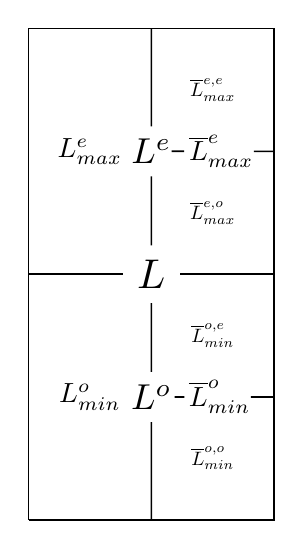
\begin{tikzpicture}[scale = .26]
		\node (L) at (0,0) [scale = 1.5]{$L$};
		\draw [semithick] (-6,0) -- (L) -- (6,0);
		\draw [semithick] (-6,-12) -- (6,-12) -- (6,12) -- (-6,12) -- (-6,-12);
		Statement
		\node (Le) at (0,6) [scale = 1.3] {$L^e$};
		\node (Lemax) at (-3,6) {$ {L}^e_{max}$};
		\node (-Lemax) at (3,6) {$\; \overline{L}^e_{max}$\!\!};
		\node at (3,3) [scale = .7] {$\overline{L}^{e,o}_{max}$};
		\node at (3,9) [scale = .7] {$\overline{L}^{e,e}_{max}$};

		\draw [semithick] (L) -- (Le) -- (0,12);
		\draw [semithick] (6,6) -- (-Lemax) -- (Le);

		\node (Lo) at (0,-6) [scale = 1.3] {$L^o$};
		\node (Lomin) at (-3,-6) {$ {L}^o_{min}$};
		\node (-Lomin) at (3,-6) {$\, \overline{L}^o_{min}$\!\!};
		\node at (3,-3) [scale = .7] {$\overline{L}^{o,e}_{min}$};
		\node at (3,-9) [scale = .7] {$\overline{L}^{o,o}_{min}$};

		\draw [semithick] (L) -- (Lo) -- (0,-12);
		\draw [semithick] (6,-6) -- (-Lomin) -- (Lo);
		\end{tikzpicture}
	\end{center}
\end{minipage}
\ \\

\begin{minipage}{.6\textwidth}
	$R = \big\{ U^0 \ot \bu.U^1 \mid U = \{u_1 < \cdots < u_{q}\} \in \P_q(n), \ \bu \in \overline{U} \big\}$ \vsk
	\begin{tab}
		$R^{e} = \{\ind_{\bu.U}(\bu) = 0\}$ \par \vsk
		\begin{tab}
			$R_{min}^{e} = \{u_q < \bu\}$ \par \vsk
			$\overline{R}_{min}^{e} = R^{e} \setminus R_{min}^{e}$ \vsk
			\begin{tab}
				$\overline{R}_{min}^{e,e} = \{\ind_{\bu.U}(r_{U}^\bu) = 0\}$ \par \vsk
				$\overline{R}_{min}^{e,o} = \{\ind_{\bu.U}(r_{U}^\bu) = 1\}$
			\end{tab}
		\end{tab} \vsk \vsk
		$R^{o} = \{\ind_{\bu.U}(\bu) = 1\}$ \par \vsk
		\begin{tab}
			$R_{max}^{o} = \{\bu < u_1\}$ \par \vsk
			$\overline{R}_{max}^{o} = R^{o} \setminus R_{max}^{o}$ \vsk
			\begin{tab}
				$\overline{R}_{max}^{o,e} = \{\ind_{\bu.U}(l_{U}^\bu) = 0\}$ \par \vsk
				$\overline{R}_{max}^{o,o} = \{\ind_{\bu.U}(l_{U}^\bu) = 1\}$
			\end{tab}
		\end{tab}
	\end{tab}
\end{minipage}
\begin{minipage}{.4\textwidth}
	\begin{center}
		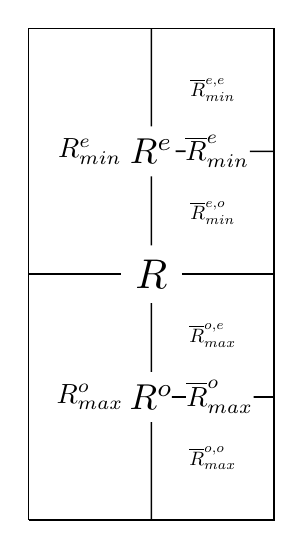
\begin{tikzpicture}[scale = .26]
		\node (L) at (0,0) [scale = 1.5]{$R$};
		\draw [semithick] (-6,0) -- (L) -- (6,0);
		\draw [semithick] (-6,-12) -- (6,-12) -- (6,12) -- (-6,12) -- (-6,-12);

		\node (Le) at (0,6) [scale = 1.3] {$R^e$};
		\node (Lemax) at (-3,6) {$ {R}^e_{min}$};
		\node (-Lemax) at (3,6) {$\overline{R}^e_{min}$\!\!};
		\node at (3,3) [scale = .7] {$\overline{R}^{e,o}_{min}$};
		\node at (3,9) [scale = .7] {$\overline{R}^{e,e}_{min}$};

		\draw [semithick] (L) -- (Le) -- (0,12);
		\draw [semithick] (6,6) -- (-Lemax) -- (Le);

		\node (Lo) at (0,-6) [scale = 1.3] {$R^o$};
		\node (Lomin) at (-3,-6) {$ {R}^o_{max}$};
		\node (-Lomin) at (3,-6) {\,$\overline{R}^o_{max}$\!\!};
		\node at (3,-3) [scale = .7] {$\overline{R}^{o,e}_{max}$};
		\node at (3,-9) [scale = .7] {$\overline{R}^{o,o}_{max}$};

		\draw [semithick] (L) -- (Lo) -- (0,-12);
		\draw [semithick] (6,-6) -- (-Lomin) -- (Lo);
		\end{tikzpicture}
	\end{center} \vsk
\end{minipage}

	
	With this notation it is a direct observation that \eqref{e:big lemma rhs w/o endpoints}, the right hand side of \eqref{e:big lemma}, is equal to \eqref{e:big lemma rhs promising}; and that the left hand side of \eqref{e:big lemma} is equal to \eqref{e:big lemma lhs}.
	
	To show that \eqref{e:big lemma rhs promising} and \eqref{e:big lemma lhs} are equal we need the following identities:
	\begin{equation} \label{e:big lemma four identities}
	\overline{R}_{min}^{e,e} = \overline{L}_{max}^{e,e}\ , \qquad
	\overline{R}_{min}^{e,o} = \overline{R}_{max}^{o,e}\ , \qquad 
	\overline{L}_{min}^{o,e} = \overline{L}_{max}^{e,o}\ , \qquad
	\overline{L}_{min}^{o,o} = \overline{R}_{max}^{o,o}.
	\end{equation}
	For a pair $U \in \P_q(n)$ and $\bu \in \overline{U}$ define when possible the sets $V^\bu_U = \{v_1 < \cdots < v_q\}$ and $W_U^\bu = \{w_1 < \cdots < w_q\}$ by
	\begin{align*}
	v_i = 
	\begin{cases}
	u_i & \text{ if } u_i \neq l_U^\bu, \\
	\bu	& \text{ if } u_i = l_U^\bu,
	\end{cases}
	\qquad \quad
	w_i = 
	\begin{cases}
	u_i & \text{ if } u_i \neq r_U^\bu, \\
	\bu	& \text{ if } u_i = r_U^\bu.
	\end{cases}
	\end{align*}
	Intuitively, $V_U^\bu$ is obtained from $U$ by replacing with $\bu$ the largest element in $U$ that is less than $\bu$.
	A similar description applies to $W_U^\bu$.
	When $U$ and $\bu$ are clear from the context we simplify notation of $V^\bu_U$ and $W^\bu_U$ to $V$ and $W$ respectively.
	Notice that
	\begin{equation*}
	l.V = \bu.U = r.W
	\end{equation*}
	and that for any $u \in \bu.U$ with $u \not \in \{l,\, \bu,\, r\}$ we have
	\begin{equation*}
	\ind_{V}(u) = \ind_{U}(u) = \ind_{W}(u).
	\end{equation*}
	We show the proof of the first identity in \eqref{e:big lemma four identities}.
	Let us consider $U^0 \otimes \bu.U^1 \in \overline{R}_{min}^{e, e}$ which by definition implies $\ind_{\bu.U}(\bu) = \ind_{\bu.U}(l_{U}^\bu) = 0$.
	This is equivalent to $\bu \in V^1$ and $l \in U^0$.
	Therefore, 
	\begin{equation*}
	U^0 \otimes \bu.U^1 =  l_{U}^\bu.V^0 \otimes V^1,
	\end{equation*}
	and since $l_{U}^\bu.V^0 \otimes V^1$ is an element in $\overline{L}_{max}^{e,e}$ we have the inclusion $\overline{R}_{max}^{e,e} \subseteq \overline{L}_{max}^{e,e}$\,.
	Similarly, the element $\bu.U^0 \otimes U^1 \in \overline{L}_{max}^{e,e}$ is equal to $W^0 \otimes r.W^1 \in \overline{R}_{min}^{e,e}$ which gives the other inclusion and proves the first identity in \eqref{e:big lemma four identities}.
	The others are proven analogously.
	
	The identities in \eqref{e:big lemma four identities} imply that
	\begin{equation} \label{e:big lemma zero sum}
	\sum_{\overline{L}_{min}^{e}} d_{\bu.U^0} \otimes d_{U^1}\ \ +\ \
	\sum_{\overline{L}_{max}^{o}} d_{\bu.U^0} \otimes d_{U^1}\ \ +\ \
	\sum_{\overline{R}_{max}^{e}} d_{U^0} \otimes d_{\bu.U^1}\ \ +\ \ 
	\sum_{\overline{R}_{min}^{o}} d_{U^0} \otimes d_{\bu.U^1}\ =\ 0,
	\end{equation}
	and, therefore, that $\eqref{e:big lemma lhs}$ is equal to \eqref{e:big lemma rhs promising} as claimed.
\end{proof}

We can now provide the proof of \cref{l:main} and of our main theorem.

\begin{proof}[Proof of \cref{l:main}]
	For any integer $i$ and $x \in X_n$ we need to prove that
	\begin{equation} \label{e:main thm proof}
	(\partial \circ \Delta_{i} + \Delta_{i} \circ \partial)(x) = (1 + T) \Delta_{i-1}(x).
	\end{equation}
	If $i < 0$ or $i > n+1$ then both sides are equal to $0$ by definition.
	If $i = 0$, the right hand side is $0$ by definition and the left hand side is $0$ since the Alexander-Whitney diagonal is a chain map.
	If $i = n+1$, then the left hand side is equal to $0$ by definition and the right hand side is equal to $(1+T) (x \otimes x) = 0$.
	Let $q = n-i$ and assume $q \not\in \{0, \dots, n-1\}$.
	We can use \cref{l:boundary of Delta} to express the left hand side of \eqref{e:main thm proof} as
	\begin{equation*}
	\sum_{\substack{U \in \P_{q}(n) \\ \bu \in \overline{U}}} \Big( d_{\bu.U^0} \otimes d_{U^1} \, + \, d_{U^0} \otimes d_{\bu.U^1} \Big) (x \otimes x),
	\end{equation*}
	whose right hand side is, thanks to \cref{l:big lemma}, equal to
	\begin{equation*}
	(1+T) \sum_{U \in \P_{q+1}(n)} d_{U^0}(x) \otimes d_{U^1}(x),
	\end{equation*}
	which by definition is $(1+T)\Delta_{i-1}(x)$.
\end{proof}